\documentclass[paper=a4, fontsize=11pt]{scrartcl} % A4 paper and 11pt font size

\usepackage[T1]{fontenc} % Use 8-bit encoding that has 256 glyphs
\usepackage{fourier} % Use the Adobe Utopia font for the document - comment this line to return to the LaTeX default
\usepackage[english]{babel} % English language/hyphenation
\usepackage{amsmath,amsfonts,amsthm} % Math packages

\usepackage{lipsum} % Used for inserting dummy 'Lorem ipsum' text into the template

\usepackage{natbib}

\usepackage{graphicx}

\usepackage{sectsty} % Allows customizing section commands
\allsectionsfont{\centering \normalfont\scshape} % Make all sections centered, the default font and small caps

\usepackage{fancyhdr} % Custom headers and footers
\pagestyle{fancyplain} % Makes all pages in the document conform to the custom headers and footers
\fancyhead{} % No page header - if you want one, create it in the same way as the footers below
\fancyfoot[L]{} % Empty left footer
\fancyfoot[C]{} % Empty center footer
\fancyfoot[R]{\thepage} % Page numbering for right footer
\renewcommand{\headrulewidth}{0pt} % Remove header underlines
\renewcommand{\footrulewidth}{0pt} % Remove footer underlines
\setlength{\headheight}{13.6pt} % Customize the height of the header

\numberwithin{equation}{section} % Number equations within sections (i.e. 1.1, 1.2, 2.1, 2.2 instead of 1, 2, 3, 4)
\numberwithin{figure}{section} % Number figures within sections (i.e. 1.1, 1.2, 2.1, 2.2 instead of 1, 2, 3, 4)
\numberwithin{table}{section} % Number tables within sections (i.e. 1.1, 1.2, 2.1, 2.2 instead of 1, 2, 3, 4)

\setlength\parindent{0pt} % Removes all indentation from paragraphs - comment this line for an assignment with lots of text

%----------------------------------------------------------------------------------------
%	TITLE SECTION
%----------------------------------------------------------------------------------------

\newcommand{\horrule}[1]{\rule{\linewidth}{#1}} % Create horizontal rule command with 1 argument of height

\title{
\normalfont \normalsize
\textsc{University of Glasgow} \\ [25pt] 
\horrule{0.5pt} \\[0.4cm] % Thin top horizontal rule
\huge Safety Critical Systems AX Report (H)\\ 
\horrule{2pt} \\[0.5cm] % Thick bottom horizontal rule
}

\author{Andrei-Mihai Nicolae\\2147392n@student.gla.ac.uk} % Your name and email

\date{\normalsize\today} % Today's date or a custom date

\begin{document}

\maketitle % Print the title

\tableofcontents % Table of contents

%----------------------------------------------------------------------------------------
%	Introduction
%----------------------------------------------------------------------------------------

\section{Introduction}

\par
Artificial Intelligence has been one of the hot topics of this decade as it is surrounding our lives more as days go by. We can see it in objects ranging from aircrafts to smart home controllers. \\

However, as AI has become so powerful, it may come with a cost for the majority of us. Because of the large number of risks when letting Artificial Intelligence and Machine Learning robots/devices perform certain actions for us (\cite{ai-risks}), we need to devote a huge amount of effort in designing better safety-oriented architectures, well-crafted and thorough testing as well as regular check-ups and revisions. Therefore, we need to see a considerable increase in tools that assess and mitigate risks when introducing AI into systems of any type. Such a tool will be discussed in further detail in this report.

%------------------------------------------------

\subsection{AI-Driven Technologies}

\par
The importance of introducing AI into a field with safety as a top priority is crucial. Because there is no human involved, the goal of the whole AI community is to let the machines actually take our place in performing certain actions, so that our tasks would be simplified. As good examples where it has become more and more developed, here is a list of examples:

\begin{itemize}
	\item Transportation (driverless cars, subways)
	\item Game playing machines (Deepmind's Go playing machine that beat the en-titre champion) \citet{deepmind}
	\item Medical robotics
	\item Manufacturing machines
	\item Education
\end{itemize}

\par
As the list can go on, we can see how AI spans throughout most of the major aspects of our lives, thus the need of careful monitoring its development.

%------------------------------------------------

\subsection{How AI Can Go Wrong}

\par
Going past the many fields driven by Artificial Intelligence nowadays, we need to also take a close look at how many technologies have proven to be very prone to failure. \\

\par
One interesting case is something that happened only a few months ago with an Uber driverless car going through a red light in front of San Francisco's Museum of Modern Art (\citet{uber-red-light}).

\par
As it was recorded on camera, the car just rushes through a busy street on red light. This is a clear sign of how developers are not placing enough testing and robust checks before launching such a safety critical systems into an open environment. \\

\par
We can see that the cause of the previous example could have been harmful for us humans. However, there have been cases where AI was involved and it was even deadly. Such an event is the killing of a Volkswagen employee who was grabbed and killed by one of the manufacturing robots in the plant (\citet{volkswagen}). Moreover, a robot in one Silicon Valley mall struck a child on the head by mistake (\citet{knightscope}). \\

\par
In conclusion, after discussing various developments in the Artificial Intelligence world and how these safety critical systems can fail drastically, a tool for assessing and mitigating such risks will be presented in the rest of this report.

%----------------------------------------------------------------------------------------
%	Tool
%----------------------------------------------------------------------------------------

\section{Tool}

\par
After extensive research, I came to the conclusion that for such an application the best technique that should be used is Model Checking adapted specifically for AI systems. \\

%------------------------------------------------

\subsection{Reasons behind Choice}

\par
Firstly, it's needed to be pointed out that various techniques (e.g. Fault Tree Analysis, Effects and Criticality Analysis) work as well for some sub-fields of AI-driven systems, but I believe that Model Checking is eventually the optimal choice. This is because of various reasons which will be exposed below.

%------------------------------------------------

\subsection{AI is Young}

\par
Because of the relatively young age of AI and ML in mainstream technology, there is quite a significant amount of improvements needed to be implemented. As shown before, there are many cases where they failed and lead to possible catastrophic outcomes. \\

\par
Model Checking is a solution to the problem: having a model system, check automatically (and exhaustively) if that particular system meets some given specification. I believe this is a very good approach to the tool needed to be implemented because the model checking applies to finite state systems (\citet{wiley-encyclopedia}). As AI is young, we need to make sure (even at the cost of time and not so optimal design decisions) that the system behaves correctly and gives the correct output regardless of the situation.

\par
As such, a technique such as Model Checking would automatically check all possible combinations and determine whether the system is prepared to use AI/ML safely or not.

%------------------------------------------------

\subsection{State of the Art Usages of the Model}

\par
There are many cases in the technology world where manufacturers and government bodies adopted Model Checking for AI-driven systems, thus making me more inclined in having confidence in the technique's effectiveness. \\

\par
One such example is how NASA used a SPIN-based Model Checker to verify the safety properties of autonomous planning systems. In their case, such an APS  would decide what a rover or spacecraft should perform next (\citet{nasa-spin}). Therefore, they needed to assure that the APS would always pick a safe choice that would not require human supervision eventually. Therefore, they came up with a solution that would replace the current empirical testing at that time (proven inefficient) with a Model Checker SPIN implementation using the Promela programming language. It proved to be very successful, being able to develop over 3 billion plans for their finite-state system. Even though this is very time-consuming and it is not optimal, as anyone can imagine, the decision a rover or a spacecraft system makes is of crucial importance, thus we can sacrifice cost for the benefit of confidence in the machine's abilities to perform the task correctly. \\

\par
Another good example is coming from the aviation field: Rockwell Collins is an important avionics and IT company that delivers safety critical systems to governmental agencies and various aircraft manufacturers. They developed 2 systems of interest to us in this report: one is called ADGS-2100 Adaptive Display and Guidance System Window Manager - it was designed to provide pilots with heads up and down displays, as well as display management software, while the other one is FCS 5000 - a new family of Flight Control Systems. \\

\begin{figure}[!ht]
    \centering
    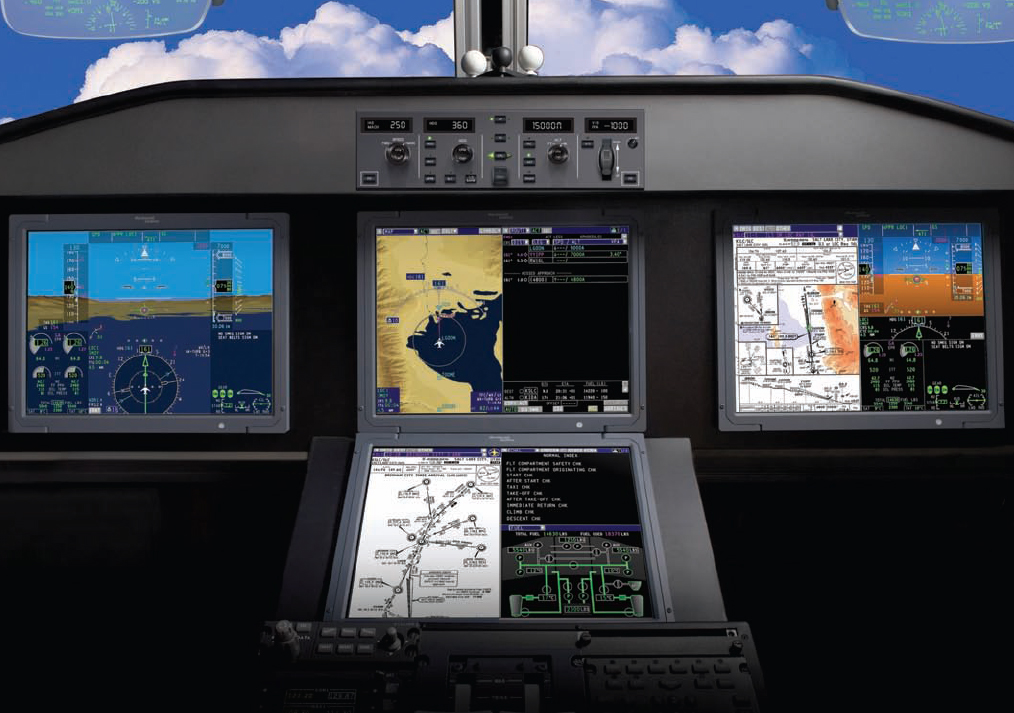
\includegraphics[width=0.8\textwidth]{display-panels.jpg}
    \caption{Pilot Display Panels}
\end{figure}

After considering various techniques to assess and mitigate risk as early and efficiently as possible, they ended up with using Model Checking (\citet{rockwell-collins}) for both applications. The systems are crucial, such that whichever would fail during a flight it would impose great risks to both pilots and other travellers. Therefore, they have imposed a Simulink specification using only Boolean and enum types (\citet{acm-model-checking}). The company has been very pleased with the approach, having 5 autonomous components which had, in turn, 563 properties developed and checked altogether. This revealed around 100 errors in early versions of the window manager. By the end of the project, however, the developers were checking properties after the design change, reporting that they were very satisfied with the new technique for assessing and mitigating risk.


%------------------------------------------------

\subsection{Available Tools}

\par
After showing how the tool is used by large companies and governmental agencies throughout the globe, there is a need to discuss about available tools to get started when applying the Model Checking technique. Because such systems where AI is becoming more involved are taking over the technology field, people need fast, reliable and easy to get started tools.

Such an example is the above-mentioned SPIN.

\begin{figure}[!ht]
    \centering
    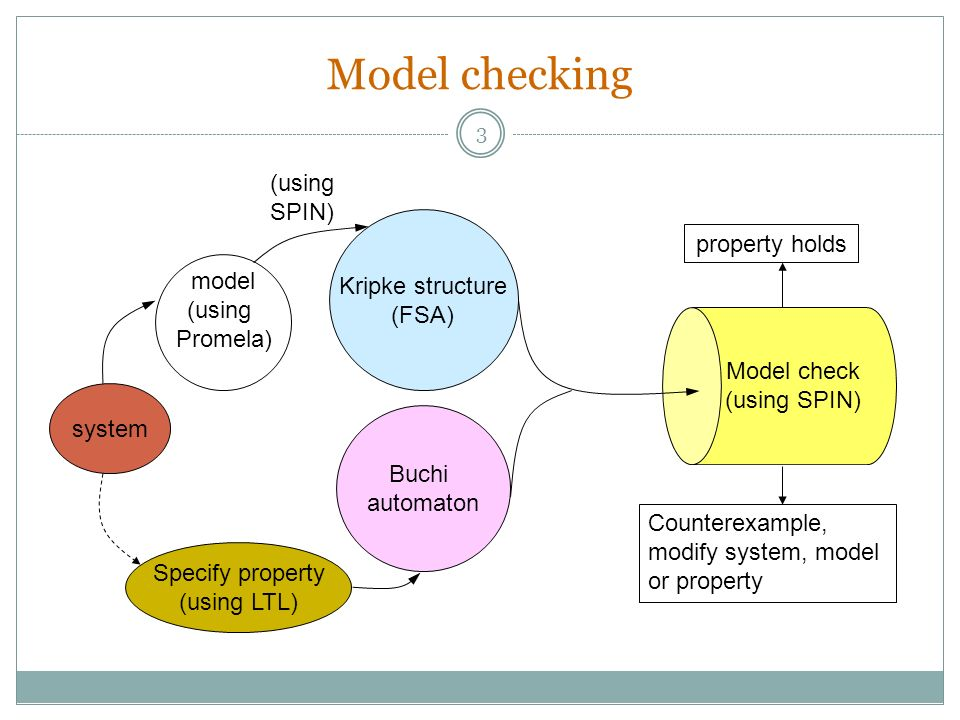
\includegraphics[width=0.8\textwidth]{spin.jpg}
    \caption{SPIN Model Checking}
\end{figure}

Not only that the model received the extremely prestigious ACM System Software Award in 2001, but it also has annual conferences held specifically for this technique. The systems need to be described in Promela language, while the properties that need to be verified are expressed as LTL (Linear Temporal Logic) formulas (\citet{spin}). \\

\par 
Apart from SPIN, NASA also made its verification tool using the Model Checking technique for the highly popular programming language Java. \\

\par
Coming to a conclusion, recent studies and developments show that there are many tools available out there that can make a developer's job to put a Model Checking technique into practice quite easy.

%------------------------------------------------

\subsection{Case Study}

\par
A specific case study that I came up with is 

%------------------------------------------------

\subsection{Implementation of the Tool}

\par
The idea I came up with was easy to implement and very efficient. As web tools are gaining more popularity among developers as days go by, the Electron framework developed by GitHub was a choice that stood out (\citet{electron}).\\

\par
Therefore, I used only web languages (JavaScript, HTML, CSS) to build a native application on all three major OS families (macOS, Windows, Linux). This was a very important design choice because I believe that websites are not such a good choice for assessing and mitigating risks in safety critical systems. This is because of a variety of reasons:

\begin{itemize}
	\item Security: having an offline application that cannot (if developed so) require an Internet connection eliminates the risks of man-in-the-middle attacks and many other techniques that might threaten the checking process and valuable information
	\item Familiarity: having an app that performs natively regardless of the specific operating system will make the developers "feel at home", becoming more productive
	\item System calls: the developers can take benefit from the system calls that can be used from within Electron 
	\item Reduced costs: as websites require server-side power and hosting, they are not a valuable option for such a tool because there would be huge costs (before we mentioned how NASA had more than 3 billion plans when running the Model Checking); however, with a standalone app, we can reduce the costs drastically as we can include the whole "server" inside the app and the local machine's resources would be used to power up the huge number of plans
\end{itemize}



%----------------------------------------------------------------------------------------
%	Evaluation
%----------------------------------------------------------------------------------------

%----------------------------------------------------------------------------------------

\section{Evaluation}

%------------------------------------------------

\subsection{Evaluation Technique}

\par
Talk about what evaluation techniques were used and why were they effective for this particular case.

%------------------------------------------------

\subsection{Iterations Progress}

\par
Talk about how the soft. dev. lifecycle went on as people were evaluated and how all steps were followed thoroughly.

%----------------------------------------------------------------------------------------
%	Results
%----------------------------------------------------------------------------------------

%----------------------------------------------------------------------------------------

\section{Results}

%----------------------------------------------------------------------------------------
%	Conclusion
%----------------------------------------------------------------------------------------

%----------------------------------------------------------------------------------------

\section{Conclusion}

\bibliographystyle{plainnat}
\bibliography{bibliography}

\end{document}

